\chapter{Sklepne ugotovitve}


% zaključek (odstavki: kaj smo naredili in kje je koda, kaj nam to omogoča, 
% kaj bi lahko še naredili)

Z izdelavo dodatka za program Orange smo zaklju"cili delo na diplomski nalogi.
Vsa koda se nahaja na prosto dostopnem repozitoriju GIT na naslovih
\url{https://github.com/zidarsk8/simple_wbd} in
\url{https://github.com/zidarsk8/orange3-data-sets}.
Dodatek je ze dostopen uporabnikom sistema Orange in ga lahko namestimo s
standardnim vmesnikom za delo z dodatki (slika \ref{addon_install}).



\begin{figure}
\begin{center}
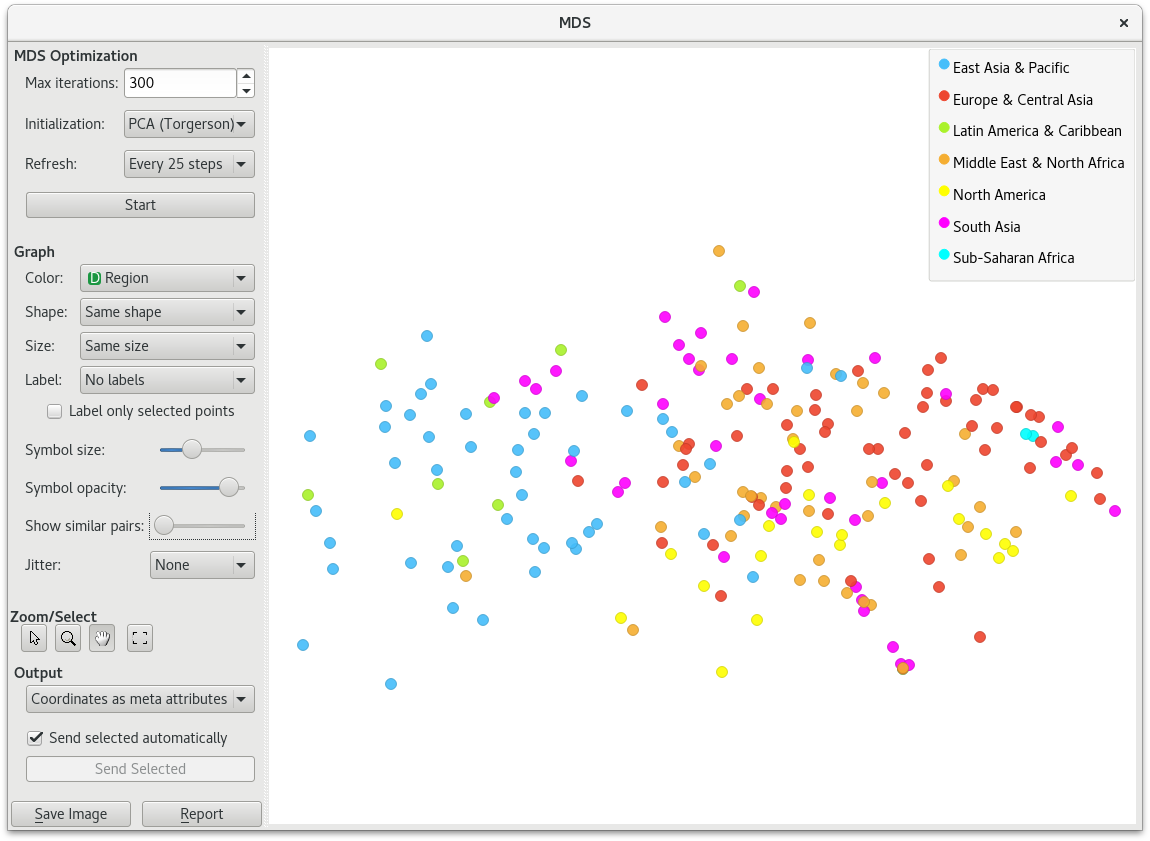
\includegraphics[width=12cm]{pic/clustering_mds.png}
\end{center}
\caption{Standardni vmesnik za delo z dodatki sistema Orange.}
\label{addon_install}
\end{figure} 




Z razvitim dodatkom smo omogo"cili dostop do podatkov programskega vmesnika Svetovne 
banke tako v grafičnem vmesniku kot v skriptnem delu programa Orange. Poleg tega
smo z našim vmesnikom tudi poenotili način dostopa do podatkov Svetovne banke
v programu Orange in s tem olajšali vzdrževanje in posodabljanje kode v
primeru spremembe programskega vmesnika Svetovne banke.



Na"s grafični dodatek za dostop do podatkov indikatorjev lahko nadgradimo tako,
da uporabnikom grafičnega vmesnika omogočimo večjo izbiro oblik izhodnih
podatkov in natančnejše presejanje rezultatov. Dodamo lahko tudi več
metapodatkov na posamezne stolpce tabele Orange, ki nam omogočijo boljšo
predstavnost v ostalih gradnikih Orange. V grafični vmesnik za dostop do
podnebnih podatkov lahko dodamo še možnost izbire vodotočnih območij meritev.
Za boljšo predstavo bi lahko postopek izbire držav, regij in vodotočnih
območij (slika \ref{climate_data_api_basins}) omogočili preko interaktivnega 
zemljevida sveta.

% - dodamo metapodatke tudi climate gradniku
% - boljsa pokritost testov
% 
% 
% - V data sets skupino bi lahko dodali se gradnik za katerega od drugih v uvodu
% nastetih spletnih programskih vmesnikov
